\chapter{Measurements}

 This chapter presents the results and program code that was used for measuring the current consumption. Some improvements was done to the program code during the measurement period, these changes are also presented in the following section.






\section{Current Consumption}

The first step was to measure the current consumption of the LoPy during a request of positional fix. Measuring of data was done outside with the measurement platform. All the measurements was done under clear sky. 


\subsection{Measurement with communication}
Program code for getting a positional fix is shown in \ref{code:intial}. The program initialize a GPIO pin that is toggled when the positional fix is acquired. The function coordinates() is from the L76 GNSS class that sets the class variable fix, when the position is received. 
\lstset{language=Python}          % Set your language (you can change the language for each code-block optionally)
\begin{lstlisting}[frame=single]  % Start your code-block

#intialize the trigger output and the Pytrack/GPS
p_out = Pin('P20', mode=Pin.OUT)
p_out.value(0)
py = Pytrack()
l76 = L76GNSS(py)
time.sleep(2)
while (True):
    #Toggle the trigger when a fix acquried
    coord = l76.coordinates()
    print ("FIX:jared ", l76.fix)
    if ((l76.fix) and not(l76.first_fix)):
        l76.first_fix = 1
        l76._set_time()
        p_out.value(1)
        time.sleep(0.25)
        p_out.value(0)
\end{lstlisting}
\label{code:intial}


After doing some measurements with the program code and analyzing it, it became evident that another power demanding task was running on the LoPy besides the GPS function.  Figure \ref{fig:startup_intial} shows the initial start up sequence of the program code.

 \begin{figure}[H]
\centering
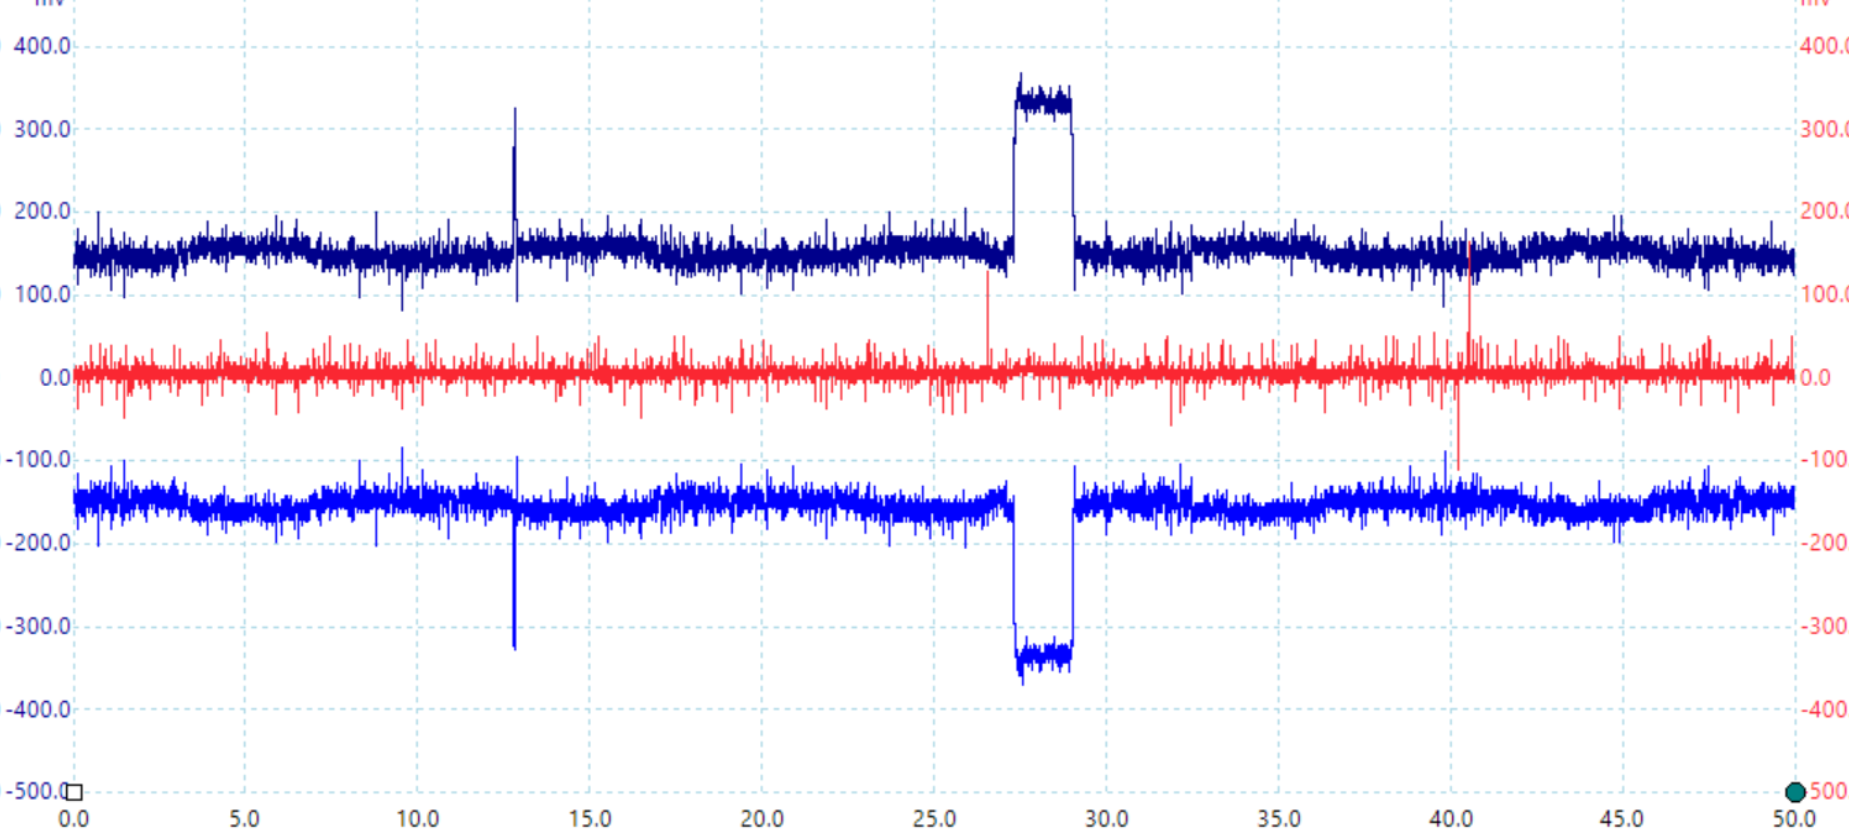
\includegraphics[width=16 cm]{Project_Report/Images/startup_intial.PNG}
\caption{Waveform of the start up sequence}
\label{fig:startup_intial}
\end{figure}


The waveform of the start up sequence have an average current of 158 mA. The conversion from the measured voltage to current is 1:1, since a 1 ohm resistor is used. The signal have an periodic surge around 320 mA. The period between the surges is around 120 ms. Table \ref{Table:WIFI_ON} shows the 20 next waveforms and their average current, and power.The periodic signal makes it difficult to explain the current consumption, as it influences the current consumption. Table \ref{Table:WIFI_ON} shows the avg current and power for the 20 next waveforms.
\begin{table}[h!]
\begin{center}
 \begin{tabular}{||c c c||} 
 \hline
 Waveform(50ms) & Avg Current(mA) & Power(mW)\\ [0.5ex] 
 \hline\hline
 1 & 158    & 24.96 \\ 
 \hline
 2 & 158    & 24.96 \\
 \hline
 3 & 152.3  & 23.19 \\
 \hline
 4 & 165.8  & 27.48 \\
 \hline
 \rowcolor{red}
 5 & 155.1  & 24.05 \\ 
 \hline
 6 & 161    & 25.92 \\ 
 \hline
 7 & 157.6  & 24.83 \\
 \hline
 8 & 149.6  & 22.38 \\
 \hline
 9 & 150    & 22.5  \\
 \hline
 10 & 143.6 & 20.62 \\ 
 \hline
 11 & 151   & 22.80 \\
  \hline
 12 & 157.3 & 24.74 \\
 \hline
 13 & 142.3 & 20.24 \\ 
 \hline
 14 & 149.8 & 22.44 \\ 
 \hline
 15 & 150.2 & 22.56 \\
 \hline
 16 & 151.2 & 22.86 \\
 \hline
 17 & 155.4 & 24.14 \\
 \hline
 18 & 142   & 20.16 \\ 
 \hline
 19 & 146   & 21.31  \\
 \hline
 20 & 192.7 & 37.13 \\[1ex]
 \hline
\end{tabular}
\end{center}
\caption{The 20 waveforms after the initial startup sequence}
\label{Table:WIFI_ON}
\end{table}

Row 5 in red, is the waveform when the receiver has a positional fix. Average current consumption is in the range[143.6-192.7] mA. This is a difference of 49.1 mA. By reviewing waveform 20, it becomes obvious that the high average current is due to the disturbance from the periodic signal. This is shown in figure \ref{fig:waveform20} 





\begin{figure}[H]
\centering
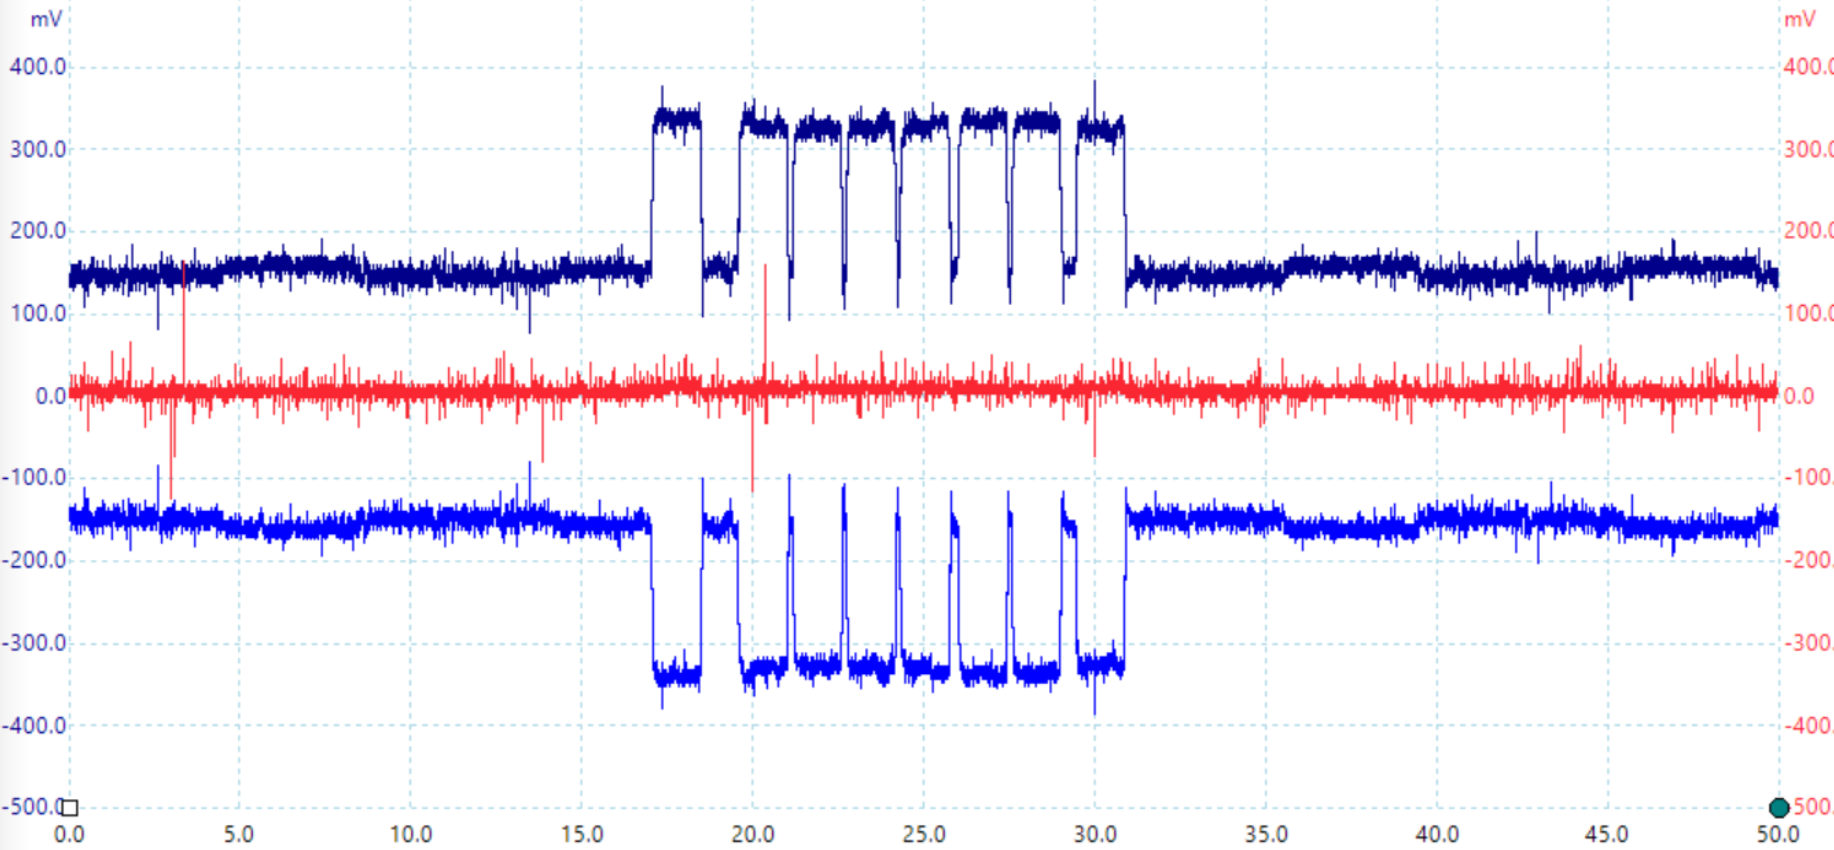
\includegraphics[width=16 cm]{Project_Report/Images/waveform20.PNG}
\caption{Waveform 20 with the inverted signal and the trigger signal(red).}
\label{fig:waveform20}
\end{figure}


\section{An improved approach}

The periodic signal is understood as the communication protocol of the WIFI and Bluetooth. The first part of the improved program code, turns the wireless protocols off to remove the disturbance. A COLD START is sent to the ARM processor to reset the GPS between each execution to remove all satellite data. A deepsleep is included after a fix has been acquired. The LoPy restarts the program code after waking up from deepsleep. 

\lstset{language=Python}          % Set your language (you can change the language for each code-block optionally)
\begin{lstlisting}[frame=single]  % Start your code-block

# initialize ``P9`` in gpio mode and make it an output
p_out = Pin('P20', mode=Pin.OUT)
p_out.value(0)
#Turn off all communication protocols
wlan= WLAN()
wlan.deinit()
bt = Bluetooth()
bt.deinit()

py = Pytrack()
l76 = L76GNSS(py)
#send cold start request
py.setup_sleep(60)
l76.write_gps(l76.COLD_START,False)
time.sleep(2)
while (True):
    coord = l76.coordinates()
    print ("FIX:jared ", l76.fix)
    if ((l76.fix) and not(l76.first_fix)):
        l76.first_fix = 1
        l76._set_time()

        p_out.value(1)
        time.sleep(0.25)
        p_out.value(0)
        py.go_to_sleep(True):

\end{lstlisting}
\label{code:intial}






\section{Measuring of deep sleep}
The time from waking up the LoPy from deepsleep until it was searching for signals in acquisition was estimated. The time was estimated by counting the number of waveforms of 200 ms that was sampled before the initializing sequence signal appeared. This time was added together with the overhead of sampling data between each waveform.19 waveforms was sampled before the initializing sequence appeared. 
\begin{equation}
200ms * 19 = 3800 ms = 3.8 s
\end{equation}
\begin{equation}
3.8 s + (20ms*19) = 4.18 s \approx  4 s
\end{equation}

The average current in deep sleep is measured to 2.3 mA. 















\section{trash}
\begin{table}[h!]
\begin{center}
 \begin{tabular}{||c c c||} 
 \hline
 Waveform(50ms) & Avg Current(mA) & Power(mW)\\ [0.5ex] 
 \hline\hline
 1 & 158    & 24.96 \\ 
 \hline
 2 & 158    & 24.96 \\
 \hline
 3 & 152.3  & 23.19 \\
 \hline
 4 & 165.8  & 27.48 \\
 \hline
 \rowcolor{red}
 5 & 155.1  & 24.05 \\ 
 \hline
 6 & 161    & 25.92 \\ 
 \hline
 7 & 157.6  & 24.83 \\
 \hline
 8 & 149.6  & 22.38 \\
 \hline
 9 & 150    & 22.5  \\
 \hline
 10 & 143.6 & 20.62 \\ 
 \hline
 11 & 151   & 22.80 \\
  \hline
 12 & 157.3 & 24.74 \\
 \hline
 13 & 142.3 & 20.24 \\ 
 \hline
 14 & 149.8 & 22.44 \\ 
 \hline
 15 & 150.2 & 22.56 \\
 \hline
 16 & 151.2 & 22.86 \\
 \hline
 17 & 155.4 & 24.14 \\
 \hline
 18 & 142   & 20.16 \\ 
 \hline
 19 & 146   & 21.31  \\
 \hline
 \rowcolor{red}
 20 & 192.7 & 37.13 \\[1ex]
\end{tabular}
\end{center}
\caption{The 20 waveforms after the initial startup sequence}
\label{Table:WIFI_ON}
\end{table}

\begin{table}[h!]
\begin{center}
 \begin{tabular}{||c c c||} 
 \hline
 Waveform(50ms) & Avg Current(mA) & Power(mw)\\ [0.5ex] 
 \hline\hline
 1 & 138.7  & 19.23 \\ 
 \hline
 2 & 130.2  & 16.95 \\
 \hline
 3 & 74.8   & 5.59  \\
 \hline
 4 & 73.22  & 5.36 \\
 \hline
 \rowcolor{red}
 5 & 72.92  & 5.31 \\ 
 \hline
 6 & 73.45  & 5.39 \\ 
 \hline
 7 & 72.63  & 5.27\\
 \hline
 8 & 73.14  & 5.39 \\
 \hline
 9 & 72.84  & 5.30 \\
 \hline
 10 & 73.83 & 5.45 \\ 
 \hline
 11 & 151   &     \\
  \hline
 12 & 157.3 \\
 \hline
 \rowcolor{red}
 13 & 142.3 \\ 
 \hline
 14 & 149.8 \\ 
 \hline
 15 & 150.2 \\
 \hline
 16 & 151.2 \\
 \hline
 17 & 155.4 \\
 \hline
 18 & 142 \\
 \hline
 19 & 146 \\
 \hline
 \rowcolor{red}
 20 & 192.7 \\ 
 [1ex]
\end{tabular}
\end{center}
\caption{The table shows wifi off}
\label{Table:WIFI_OFF}
\end{table}

\newpage